%             
% Hall D Note
% 
\documentclass[12pt]{article}


\usepackage{color}

% ===    Set a true/false value for PDF hyper marks  

\newif\ifhyprf
%\hyprffalse   
\hyprftrue

\RequirePackage{ifpdf}
  
\ifpdf
    \pdfoutput=1        % we are running PDFLaTeX
    \pdftrue
\else
    \pdffalse           % we are not running PDFLaTeX
\fi

\ifpdf
  \pdfcompresslevel=9
  \usepackage[pdftex]{graphicx}
%  \usepackage{thumbpdf}
  \definecolor{rltred}{rgb}{0.75,0,0}
  \definecolor{rltgreen}{rgb}{0,0.3,0}
  \definecolor{rltblue}{rgb}{0,0,0.75}
  \definecolor{rltdarkgreen}{rgb}{0.1,0.6,0.1}
  \ifhyprf
     \usepackage[pdftex,
         colorlinks=true,
         urlcolor=rltblue,       % \href{...}{...} external (URL)
         filecolor=rltgreen,     % \href{...} local file
         linkcolor=rltred,       % \ref{...} and \pageref{...}
         citecolor=rltdarkgreen, % citations
         pagebackref,
         pdfpagemode=None,
         pdftitle={Civil Reference Concepts for BDX},
         pdfauthor={many},
         pdfsubject={Civil Reference Concepts for BDX},
         pdfkeywords={JLab Beam Dump Experiment}]{hyperref}
  \fi
  \usepackage{pdfcolmk}
  \DeclareGraphicsExtensions{.pdf,.png,.jpg}
\else
  \usepackage{graphicx}
  \DeclareGraphicsExtensions{.eps,.epsi,.ps,.eps.gz,.epsi.gz,.ps.gz}
\fi

\setlength{\textwidth}{6.0in}
%\setlength{\textheight}{9.5in}
\setlength{\textheight}{8.75in}
\setlength{\evensidemargin}{0.25in}
\setlength{\oddsidemargin}{0.25in}
\setlength{\topmargin}{-0.25in}
\setlength{\footskip}{0.25in}
%\setlength{\parindent}{0pt}
%\setlength{\parskip}{0in}
\usepackage{graphicx,lscape,rotating}
\pagenumbering{arabic}
%\input epsf
\usepackage[utf8]{inputenc}

\begin{document}

\begin{flushright}
GlueX-doc-5506\\
github: eltonssmith/reports/CPP\_PID\_systematics\\
February 28, 2022
\end{flushright}



%\pagestyle{myheadings}
%\markright{BDX-NOTE-2015-002}

%%%%%%%%%%%%%%%%%%%%%%%%%%%%%%%%%  TITLE %%%%%%%%%%%%%%%%%%%%%%%%%%%%%%%%
\begin{center}
{\Large \bf Toy Model for PID systematics in CPP}\\*[0.5cm]
\end{center}
%%%%%%%%%%%%%%%%%%%%%%%%%%%%%%%  AUTHORS %%%%%%%%%%%%%%%%%%%%%%%%%%%%%%%% 

\begin{center}   
{\sc  E.S. Smith}\\  
\end{center}

%\tableofcontents

\section{Introduction}
We are in the process of clarifying the requirements for the multi-variate analysis (MVA) that will be used to determine the number
of $\pi^+\pi^-$ events in the data sample collected by the CPP experiment \cite{CPPexp}.  The pion pairs will be collected along with 
a large number of Bethe-Heitler $\mu^+\mu^-$ events that are produced with 10$\times$ the cross section. The ratio of cross sections is 
denoted by $\beta\approx 10$. In this sample dominated by muon pairs, we must determine the number of pions with high precision
and, at the same time, have a high rejection of muons. This is the goal of the MVA. 

The purpose of the present study is to provide guidelines for the requirements of the MVA that achieve the goals of the experiment. In Fig.\,\ref{fig:Proposal_Table2} 
we reproduce Table~2 of the experimental proposal, which contains a summary of the error budget for the experiment. CPP aims to determine
the $\pi^+\pi^-$ Primakoff cross section with a precision of 1.5\%. This uncertainty is dominated by contributions other than the $\pi/\mu$ 
particle-identification (PID) analysis that is the focus of this note. We propose that, in order to achieve the final experimental uncertainty, 
we limit all non-dominant contributions to the error budget to be less than 0.5\%. Added in quadrature, this would increase the overall uncertainty to only 1.58\%. 

\begin{figure}[tbph]
\begin{center}
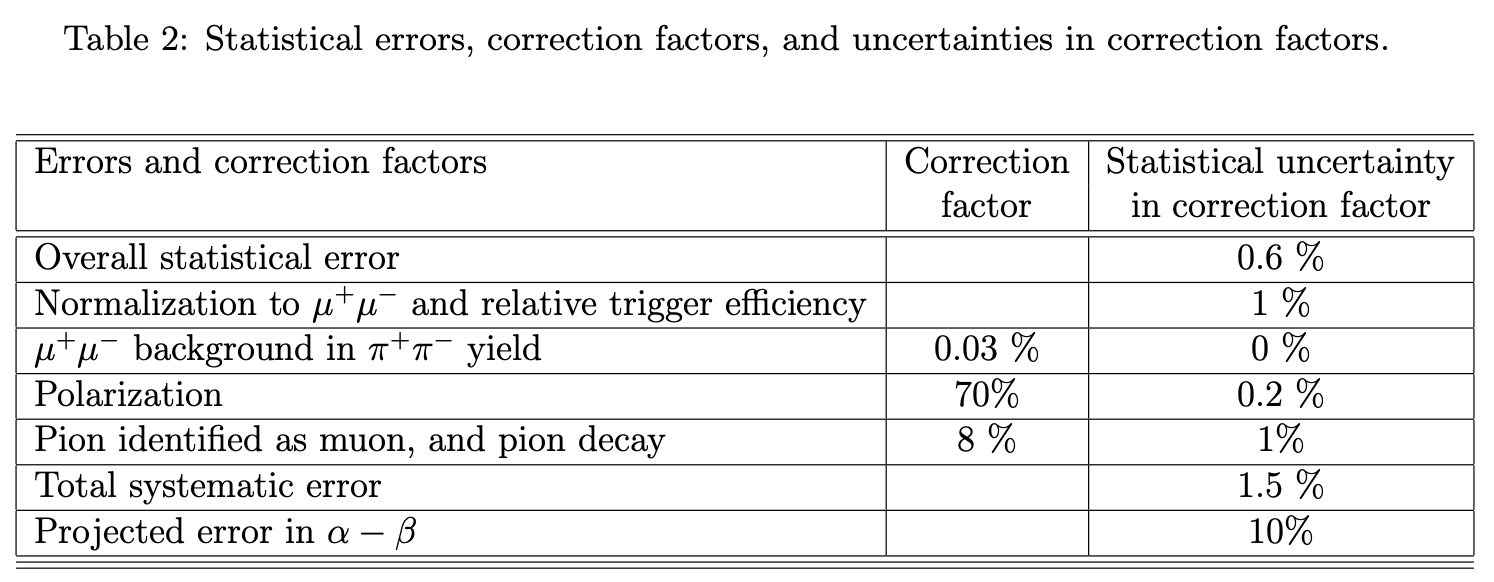
\includegraphics[height=6cm,clip=true]{Proposal_Table2}
\caption{Table 2 from the CPP Proposal \cite{CPPexp}. The goal of the experiment is to determine the Primakoff cross section with
an accuracy of 1.5\%. At the time of the proposal, the main contributors to the error budget were the overall statistical uncertainty, the absolute
normalization and the systematic uncertainty from pions identified as muons. The present study addresses a non-dominant systematic of 
$\pi/\mu$ particle identification.
\label{fig:Proposal_Table2}}
\end{center}
\end{figure} 

\section{Toy model}
We present a toy model for the MVA in order to gain insight into relevant dependencies that may contribute to the systematic uncertainty.  The model outlined schematically in Fig.\,\ref{fig:toy_systematics_c1}. For the purpose of this study, we assume the MVA analysis is conducted using entire events, i.e. not per particle. Each event would contain two charged particles, either two pions or two muons. In this context, the term pions or muons refers to the particle pairs. The MVA boils down all the information about pion and muon events into a single discriminating variable $\alpha$ (the ``MVA response'') which allows one to reject most of the muons while keeping a large fraction of pions.

The MVA responses to pions and muons in this toy model are shown in Fig.\,\ref{fig:toy_systematics_c1} as red and blue curves on linear and logarithmic scales. The curves in this toy model are taken to be exponentials for ease of plotting and manipulation. Particle identification is tuned by selecting a particular value of the response variable 
$\alpha_{cut}$. Events with a value of $\alpha$ below this cut preferentially select pions and reject muons. For this study we have chosen
$\alpha_{cut}=0.674$ such that the fraction of pion pairs below the cut is $\epsilon_{\pi} = 0.95$. The corresponding fraction of muon pairs below this cut 
is $\epsilon_{\mu} = 1.5 \times 10^{-3}$.

\begin{figure}[tbph]
\begin{center}
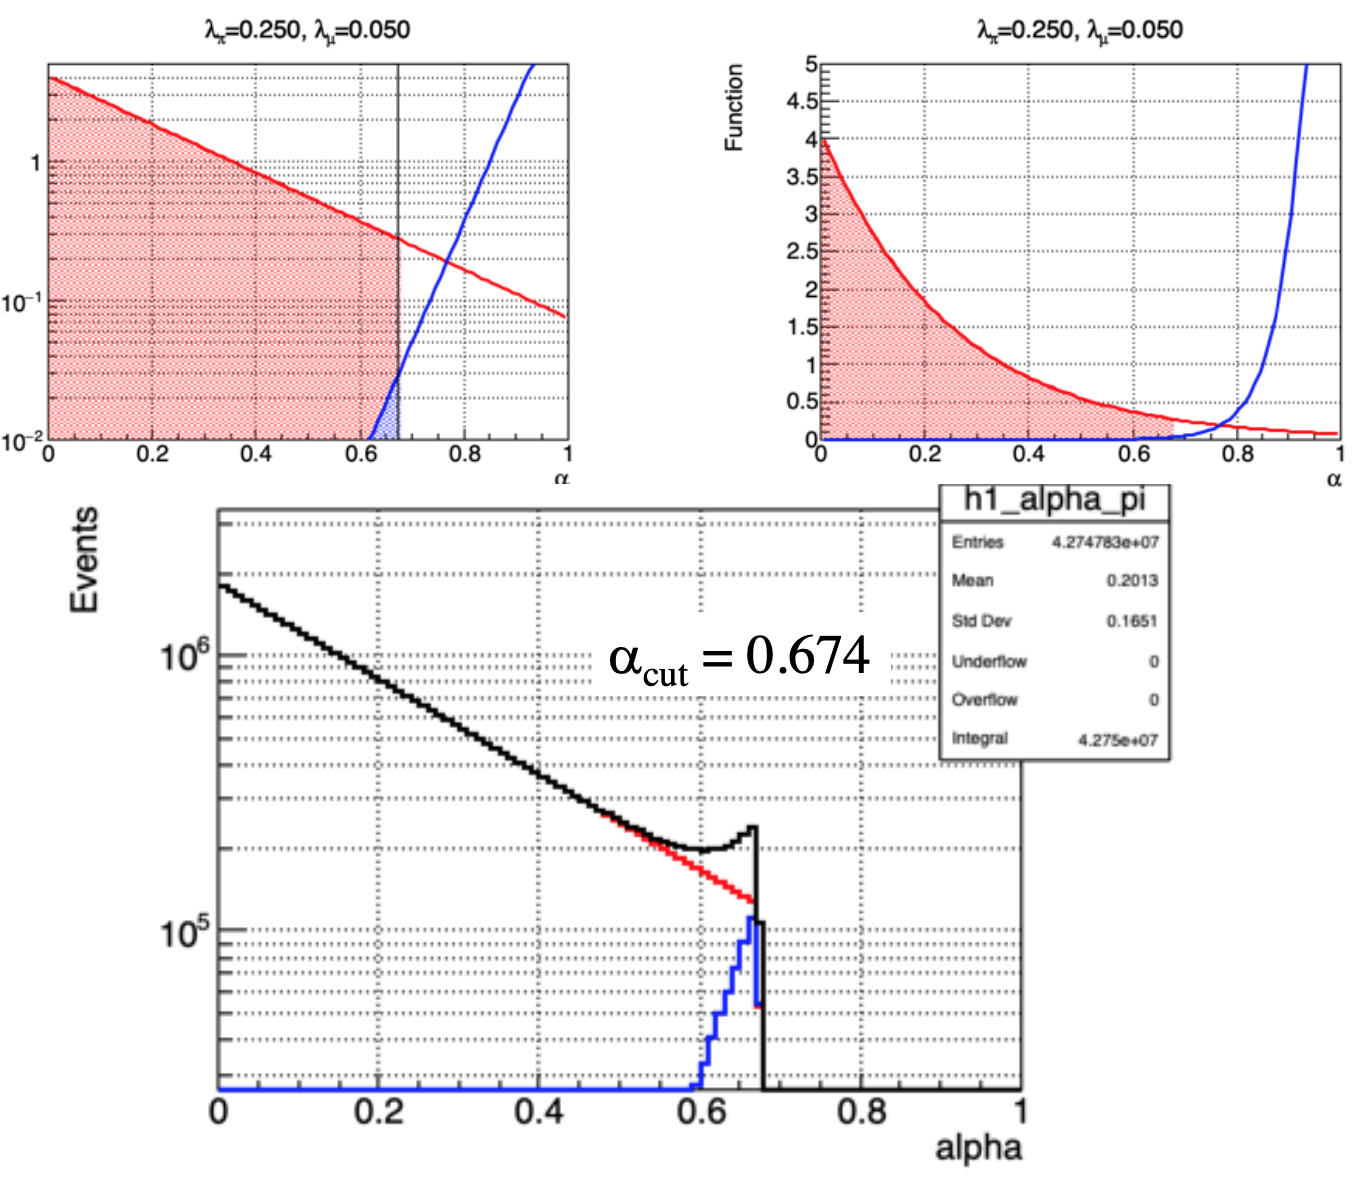
\includegraphics[height=12cm,clip=true]{toy_systematics_c1}
\caption{Toy model for the MVA response. Top Left) Pion function (red), muon function (blue) with a vertical logarithmic scale. 
Top right) Pion function (red) and muon function (blue) with a vertical linear scale.
Bottom) Histogram of the distribution of 25,000 pion and 250,000 muon ``events" generated. Only ``events" below the selection ($\alpha < \alpha_{cut}$) 
are plotted as a function of the randomly distributed MVA response ($\alpha$). The MVA response is taken for $\alpha_{cut}=0.674$. 
The total number of events below the cut is in black, pions in red and muons in blue.
\label{fig:toy_systematics_c1}}
\end{center}
\end{figure} 

\section{Dependencies}
In this section we investigate the uncertainty created in the extracted number of pion events from imprecise knowledge regarding the effect of the MVA selection on the true fractions of pions and muons selected using a particular value of $\alpha_{cut}$. In this study we attribute all the uncertainty of the selected fractions on our imprecise knowledge of the value of $\alpha_{cut}$, while equivalently the selection cut could be known but the response functions are imperfectly known. 
We start with some basic definitions. We take the number of events in our sample (selected by the cut) to be $\mathbf{ N_m  =  \epsilon_\pi N_\pi + \epsilon_\mu N_\mu}$, where the ``m" will refer to ``measured" quantities.  The number of pions, $N_\pi$, and number of muons, $N_\mu$, correspond to the total number of pions and muons without the selection cut and the fractions $\epsilon_\pi$ and $\epsilon_\mu$ contain the effect of the selection. This sample is a mixture of pion and muon events. Our best estimate of the total number of pions is given by 
\begin{eqnarray}
N_\pi^m & = & {N_m - \epsilon_\mu N_\mu \over \epsilon_\pi}.
\end{eqnarray}
Assuming we know the overall ratio between pions and muons, we have $N_\mu  =  \beta N_\pi$.
%\begin{eqnarray}      
%N_\pi^m & = & {N_m - \epsilon_\mu \beta N_\pi \over \epsilon_\pi}
%\end{eqnarray}
Since $\epsilon_\mu \leq 10^{-3}$ (small), we may substitute $N_\pi \sim N_m/\epsilon_\pi$ in the second term to obtain the following equation for the estimated number of pions in the sample:
\begin{eqnarray}
N_\pi^m & = & \left(N_m \over \epsilon_\pi \right) \left(1 - { \beta \over \epsilon_\pi} \epsilon_\mu \right).   \label{eq:npi_m}
\end{eqnarray}
We study how the uncertainties in $\epsilon_\pi$ and $\epsilon_\mu$ affect the estimated number of pions. For this study, the total number of pions $N_\pi$ and the parameter $\beta$ are taken to be constant. These latter quantities will, of course, contribute to the overall experimental statistical and systematic uncertainties. For example, the uncertainties in $N_\pi$ are closely related to the first two entries in the table in Fig.\,\ref{fig:Proposal_Table2} but are not considered in this study.
By making some reasonable approximations, one can write the changes in $N_\pi^m$ due to uncertainties in $\epsilon_\pi$ and $\epsilon_\mu$ as 
\begin{eqnarray}
\delta N_\pi^m \over N_\pi^m & = & {\delta \epsilon_\pi \over \epsilon_\pi} \left( 1 + {\epsilon_\mu \beta \over \epsilon_\pi} \right)
\approx {\delta \epsilon_\pi \over \epsilon_\pi}     \label{eq:delta_pi}
\end{eqnarray}
and
\begin{eqnarray}
\delta N_\pi^m \over N_\pi^m  & = & {\beta \over \epsilon_\pi} \delta \epsilon_\mu .     \label{eq:delta_mu}
\end{eqnarray}

\section{Toy Monte Carlo}
We perform ``toy experiments" in the following way: We generate 25,000 values of $\alpha$ for pion events and 
250,000 values of $\alpha$, assuming $\beta=10$, for muon events according to the MVA distributions shown in Fig.\,\ref{fig:toy_systematics_c1}. The number of events below cut ($N_m$) is computed based on the generated values of $\alpha$.  The estimated number of pions ($N_\pi^m$) is then calculated using Eq.\,\ref{eq:npi_m} with $N_m$ as an input and assuming a constant known value for $\beta$. The values of $\epsilon_\pi$ and $\epsilon_\mu$ used in the calculation are varied systematically to investigate how the estimated number of pions ($N_\pi^m$) changes. We note that the event generation uses $\alpha_{cut}=0.674$ in all cases, which corresponds to a generated values of $\epsilon_\pi=0.95$ and $\epsilon_{\mu} = 1.48 \times 10^{-3}$. However, the estimated number of pions will vary depending on what fraction of events are assumed to lie below the cut, simulating the uncertainty in the knowledge of $\alpha_{cut}$. 

In Fig.\,\ref{fig:cpp_systematics_lpi025_lmu005_c2} we study the dependence of the estimated number of pions on the assumed value of $\epsilon_\pi$. In Fig.\,\ref{fig:cpp_systematics_lpi025_lmu005_c3} we study the dependence of the estimated number of pions on the assumed value of $\epsilon_\mu$. In each case, the other variable is used at the generated value.  In each panel we plot the difference between the estimated number of pions  using Eq.\,\ref{eq:npi_m} and the total number of pions (fixed at 25,000). There are 100 entries per panel, each corresponding to the generation of 25,000 pions and 250,000 muon values of $\alpha$, which are used to determine $N_m$ for each ``experiment." The number of pions in each ``experiment" was chosen to correspond to the approximate number of pion pairs expected for the CPP experiment. 

As an aside, we note that there is a statistical variation due to how events fall above or below the cut $\alpha_{cut}$ that is on the order of 40 events out of 25,000 pions, or 0.16\%.  This statistical effect shows up as a width of the distributions in the plots, even though the total number of generated events is fixed. The effect is certainly small, but not zero.

In Fig.\,\ref{fig:cpp_systematics_lpi025_lmu005_c4} we summarize the results of the plots in Figs.\,\ref{fig:cpp_systematics_lpi025_lmu005_c2} and \ref{fig:cpp_systematics_lpi025_lmu005_c3}, where the mean of each histogram is plotted as a function of the assumed value for $\alpha_\pi$ (top plot) or as a function of the assumed value of $\alpha_\mu$ (bottom plot). The response as a function of both variables is quite linear, as might be expected from Eqs.\,\ref{eq:delta_pi} and \ref{eq:delta_mu}. The horizontal lines on the plot display the proposed constraint on the uncertainty in $\delta N_\pi^m / N_\pi^m$ of 0.5\%. This behavior represents the systematic variation in this toy model from changes in $\epsilon_\pi$ and $\epsilon_\mu$.

\section{Discussion}
If we require that the systematic uncertainty in the MVA-response cut 
contribute to $\delta N_\pi^m$/$N_\pi^m <$~0.5\%, as suggested in the introduction, then from
Eqs.\,\ref{eq:delta_pi} and \ref{eq:delta_mu} we can derive the following requirements (assume $\epsilon_\pi\approx 1$):
\begin{eqnarray}
\delta \epsilon_\pi & < & 0.005 \, \epsilon_\pi   \approx 0.005 \\      \label{eq:req_pi}
\delta \epsilon_\mu  & < & 0.005 \,\beta \,\epsilon_\pi = 0.0005 \, \epsilon_\pi.   \approx 0.0005  \label{eq:req_mu}
\end{eqnarray}
These conditions constrain the uncertainties of $\epsilon_\pi$ and $\epsilon_\mu$, not the values themselves. Therefore, in order to pick target values for $\epsilon_\pi$ and $\epsilon_\mu$, we must resort to additional considerations.  The part of the pion spectrum above $\alpha_{cut}$ is buried under the muon background and therefore will be the hardest to assess quantitatively. In addition, the uncertainty in determining the number of pions below $\alpha_{cut}$ will be tied to the overall normalization of the experiment. Therefore, we propose we use the fractional uncertainty in the number above the cut to constrain $\alpha_\pi$:
\begin{eqnarray}
{\delta \epsilon_\pi \over 1 - \epsilon_\pi} & < & 0.1 \rightarrow \epsilon_\pi \geq 0.95.
\end{eqnarray}
By the same reasoning, we propose using the fraction of muons below the cut, i.e. the muon contamination, as a guide for constraining $\epsilon_\mu$: 
\begin{eqnarray}
{\delta \epsilon_\mu \over \epsilon_\mu} & < & 1/3 \rightarrow \epsilon_\mu \leq 0.0015.
\end{eqnarray}
The conditions on the fractional uncertainties are based on experience; the target uncertainty for $\epsilon_\mu$ was chosen looser than for $\epsilon_\pi$ since the 
absolute values are smaller.
These targets have been used as the mean values in the toy simulations and presented in Fig.\,\ref{fig:cpp_systematics_lpi025_lmu005_c4}. Of course all these are soft constraints and tradeoffs are possible based on other considerations. 

\begin{landscape}
\begin{figure}[tbph]
\begin{center}
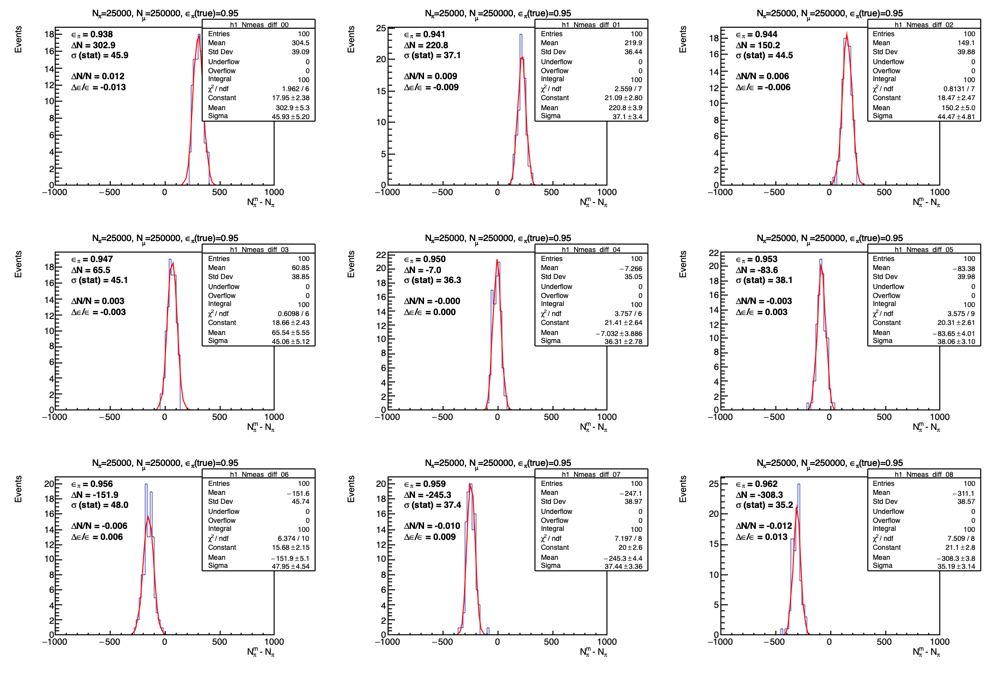
\includegraphics[height=14cm,clip=true]{cpp_systematics_lpi025_lmu005_c2}
\caption{Each panel is the result of 100 ``experiments," where pion and muon events are generated with $\epsilon_\pi=0.95$. The estimated number of pions is calculated and then histogramed based on an assumed value of $\epsilon_\pi$ that varies from panel to panel. The assumed value of $\epsilon_\pi$ ranges from 0.938 $-$ 0.962, while the value of  $\epsilon_\mu$ is fixed at its generated value. The central panel shows the estimated number of pions calculated using the generated value of $\epsilon_\pi$ and therefore is centered on zero.
The width of the distribution is statistical in nature due to the random generation of $\alpha$ even though the total number of pions without the selection cut is fixed. 
\label{fig:cpp_systematics_lpi025_lmu005_c2}}
\end{center}
\end{figure} 
\end{landscape}

\begin{landscape}
\begin{figure}[tbph]
\begin{center}
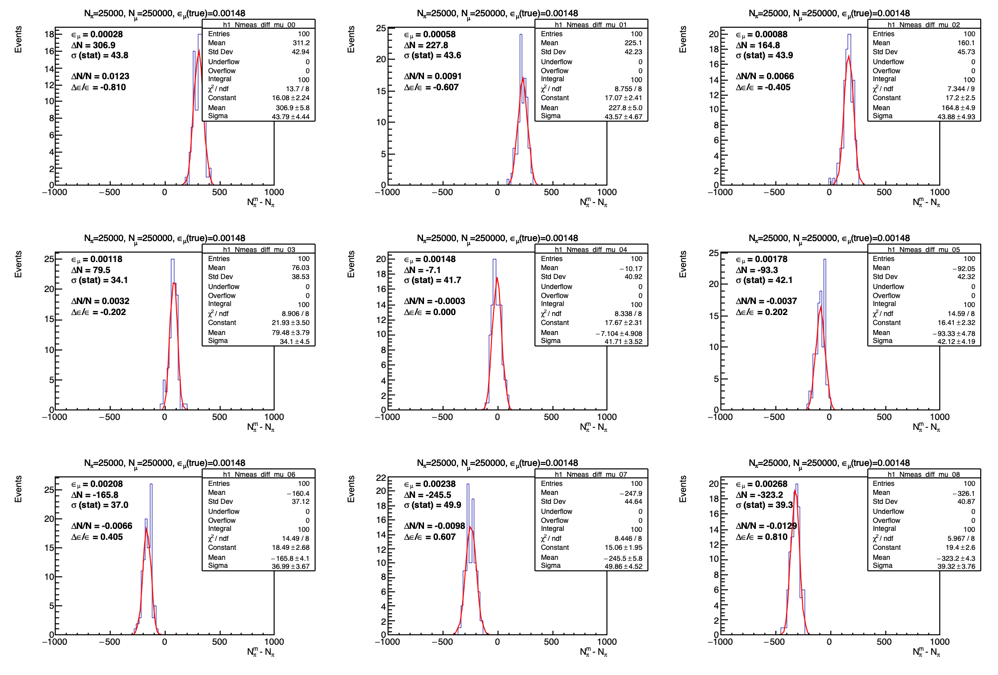
\includegraphics[height=14cm,clip=true]{cpp_systematics_lpi025_lmu005_c3}
\caption{Each panel is the result of 100 ``experiments," where pion and muon events are generated with $\epsilon_\mu=1.48 \times 10^{-3}$. The estimated number of pions is calculated and then histogramed based on an assumed value of $\epsilon_\mu$ that varies from panel to panel. The assumed value of $\epsilon_\mu$ ranges from 0.00028 $-$ 0.00268, while the value of  $\epsilon_\pi$ is fixed at its generated value. The central panel shows the estimated number of pions calculated using the generated value of $\epsilon_\mu$ and therefore is centered on zero.
The width of the distribution is statistical in nature due to the random generation of $\alpha$ even though the total number of pions without the selection cut is fixed. 
\label{fig:cpp_systematics_lpi025_lmu005_c3}}
\end{center}
\end{figure} 
\end{landscape}


\begin{figure}[tbph]
\begin{center}
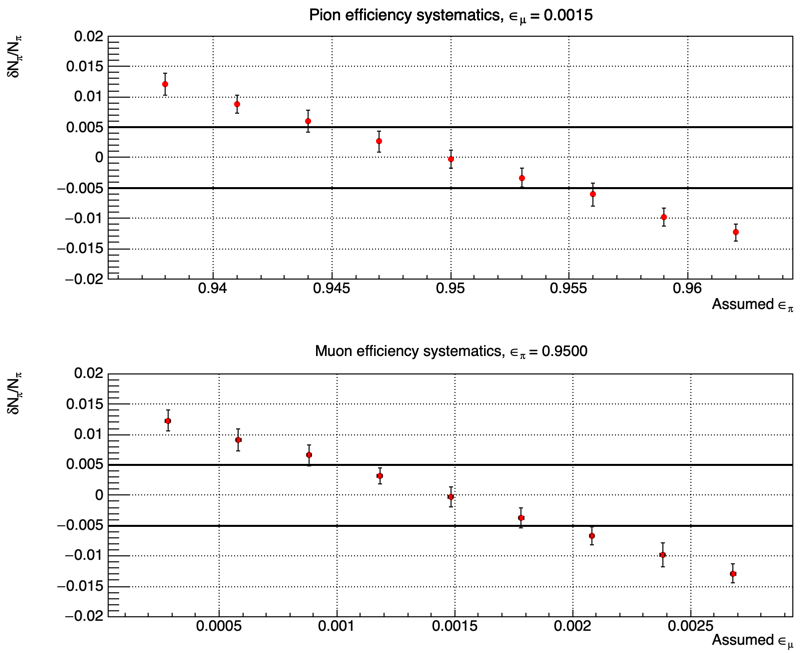
\includegraphics[height=12cm,clip=true]{cpp_systematics_lpi025_lmu005_c4}
\caption{Top) Systematic variation of the estimated number of pions as a function of the assumed value of $\epsilon_\pi$ in the calculations.
Bottom) Systematic variation of the estimated number of pions as a function of the assumed value of $\epsilon_\mu$ in the calculations.\label{fig:cpp_systematics_lpi025_lmu005_c4}}
\end{center}
\end{figure} 


%\nocite{*}
\bibliographystyle{unsrt}
\bibliography{CPP_PID_systematics}

\end{document}
